% Original link - ShareLaTeX blog:
%
%   https://www.sharelatex.com/blog/2013/08/29/tikz-series-pt3.html
%
\documentclass[10pt]{article}
\usepackage{amsmath}
\usepackage[margin=2cm]{geometry}
\parindent = 0.0in
\usepackage{color}
\usepackage{graphicx}
\usepackage{tikz}
\usetikzlibrary{shapes.geometric, arrows, backgrounds}

\tikzstyle{startstop} = [rectangle, rounded corners, minimum width=1.5cm,
                         minimum height=4mm, text centered, draw=black, 
                         fill=red!30]

\tikzstyle{loopstart} = [rectangle, rounded corners, minimum width=1.5cm,
                         minimum height=4mm, text centered, draw=black, 
                         fill=cyan!20]

\tikzstyle{process}   = [rectangle, minimum width=1.5cm, minimum height=4mm, 
                         text centered, draw=black, fill=orange!30]

\tikzstyle{bgframe}   = [rectangle, minimum width=1.5cm, minimum height=4mm, 
                         text centered, draw=black, fill=orange!10]

\tikzstyle{decision}  = [diamond, minimum width=2.5cm, minimum height=2mm, 
                         text centered, draw=black, fill=green!30]

\tikzstyle{io} = [trapezium, trapezium left angle=70, 
                  trapezium right angle=110, minimum width=1.5cm, 
                  minimum height=4mm, text centered, draw=black,
                  fill=blue!30]

\tikzstyle{point} = [rectangle, text centered, draw=white]

\tikzstyle{arrow} = [thick,->,>=stealth]
\tikzstyle{line}  = [thick]

\begin{document}
\subsection*{Flowchart of adaptive timestepping in {\tt driver.f90}}

\vspace{1cm}


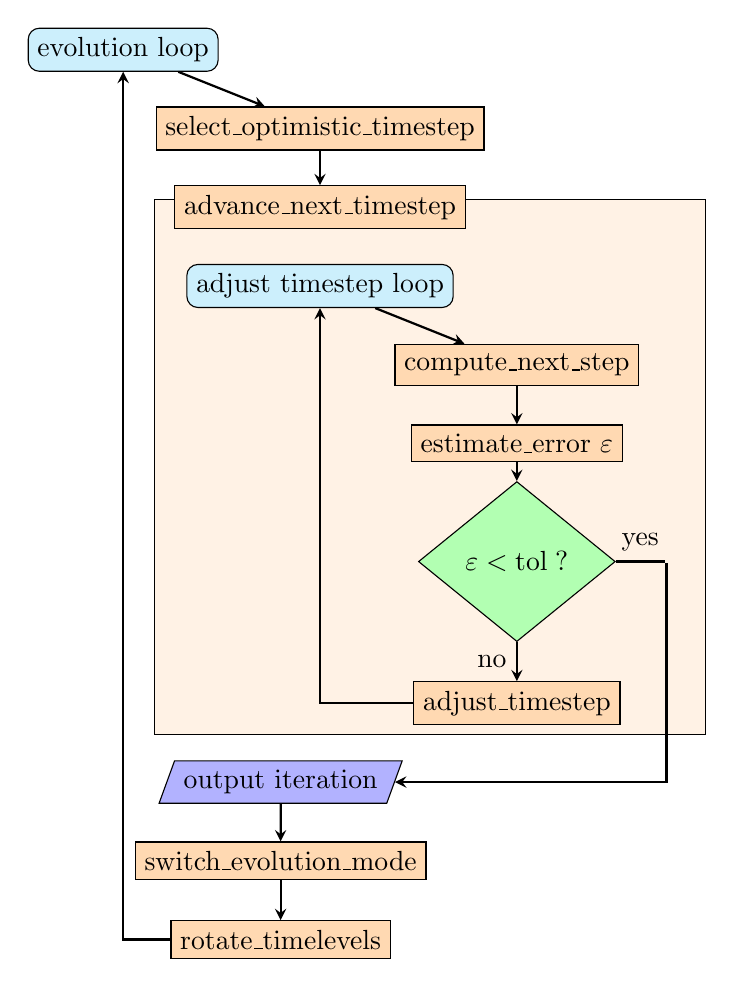
\begin{tikzpicture}[node distance=1.0cm]
\node (ev)  [loopstart] {evolution loop};
\node (sel) [process,   below of=ev,   xshift= 2.5cm] {select\_optimistic\_timestep};
\node (adv) [process,   below of=sel]                 {advance\_next\_timestep};
\node (alp) [loopstart, below of=adv]                 {adjust timestep loop};
\node (com) [process,   below of=alp,  xshift= 2.5cm]   {compute\_next\_step};
\node (est) [process,   below of=com]                   {estimate\_error $\varepsilon$};
\node (tol) [decision,  below of=est,  yshift=-0.5cm]   {$\varepsilon < {\rm tol}\;$?};
\node (adj) [process,   below of=tol,  yshift=-0.8cm]   {adjust\_timestep};
\node (out) [io,        below of=adj,  xshift=-3.0cm] {output iteration};
\begin{scope}[on background layer]
  \node (pt1) [point,     right of=tol,  xshift= 1.0cm] {};
  \node (pt2) [point,     right of=pt1,  xshift=-11mm, yshift= 1mm] {};
\end{scope}
\node (swi) [process,   below of=out]                 {switch\_evolution\_mode};
\node (rot) [process,   below of=swi]                 {rotate\_timelevels};
\begin{scope}[on background layer]
  \node (ant) [bgframe, below of=adv, xshift=1.4cm, yshift=-2.3cm, 
               minimum width=7cm, minimum height=6.8cm]  {};
\end{scope}

\draw [arrow] (ev)  -- (sel);
\draw [arrow] (sel) -- (adv);
\draw [arrow] (alp) -- (com);
\draw [arrow] (com) -- (est);
\draw [arrow] (est) -- (tol);
\draw [arrow] (tol) -- node[anchor=east]{no} (adj);
\draw [arrow] (adj) -| (alp);
\draw [line]  (tol) -- node[anchor=south, xshift= 0.0cm]{yes} (pt1);
\draw [arrow, xshift=-0.5cm] (pt2) |- (out);
\draw [arrow] (out) -- (swi);
\draw [arrow] (swi) -- (rot);
\draw [arrow] (rot) -| (ev);
\end{tikzpicture}

%  \includegraphics[height=0.2\textheight]{semistructured}

\end{document}
